
\documentclass[12pt]{article}
\usepackage{amsmath}
\usepackage{amssymb}
\usepackage{framed}
\usepackage{graphicx}
\voffset=-1.5cm
\oddsidemargin=0.0cm
\textwidth = 470pt

\begin{document}
\author{Kevin O'Brien}
\title{Cluster Analysis - k-means Clustering}
\Large
\tableofcontents
\newpage

\section{k-Means Clustering}
\tableofcontents
\newpage %=========================================== %
\subsection{Differences between K-means and Hierarchical Clustering}
\begin{itemize}
\item \textbf{Complexity of Proximity Matrix} \\  Hierarchical clustering requires a distance or similarity matrix between all pairs of cases. That's an extremely large matrix if you have tens of thousands of cases in your data .

\item A clustering method that doesn't require computation of all possible distances is \textbf{\textit{k-means clustering}}. This approach differs from hierarchical clustering in several ways. Perhaps the most important of these ways is that you have to know in advance the number of clusters you want. 
\item You can't get solutions for a range of cluster numbers unless you rerun the analysis for each different number of clusters.

\item The algorithm is called \textbf{k-means}, where \textbf{k} is the number of clusters you want, since a case is assigned to the cluster for which its distance to the \textbf{\textit{cluster mean}} is the smallest.


\item The k-means algorithm repeatedly reassigns cases to clusters, so the same case can move from cluster to cluster during the analysis. \\On the other hand, in hierarchical clustering, cases are added only to existing clusters. They are permanently assigned to their particular cluster (in as far as that makes sense in the context of hierarchical clustering), with a widening circle of ``neighbours".

\newpage



\item \textbf{Computational Differences}: \\ The k-means algorithm follows an entirely different concept than the hierarchical methods
discussed before.\\ This algorithm is not based on distance measures such as
Euclidean distance or city-block distance, but uses the \textbf{\textit{within-cluster variation}} as a measure to form homogenous clusters. 
\item 
Specifically, the procedure aims at segmenting
the data in such away that the within-cluster variation is minimized.\\ Consequently, we
do not need to decide on a distance measure in the first step of the analysis.

\item The action in the algorithm centers around finding the k-means. You start out with an initial set of means and classify cases based on their distances to the centers.

\item Next, you compute the cluster means again, using the cases that are assigned to the cluster; then, you reclassify all cases based on the new set of means. You keep repeating this step until cluster means don't change much between successive steps.

\item Finally, you calculate the means of the clusters once again and assign the cases to their permanent clusters.
\end{itemize}
%------------------------------------------------------------------%
\newpage
\subsection{Implementation with \texttt{R}}
\begin{itemize}
\item The \texttt{kmeans()} Command\\
The format of the k-means function in \texttt{R} is \texttt{kmeans(x, centers)} where x is a \textbf{numeric} dataset (matrix or data frame) and \texttt{centers} is the number of clusters to extract. \item The function returns the cluster memberships, centroids, sums of squares (within, between, total), and cluster sizes.
\end{itemize}

\subsection{The k-Means Algorithm}
\begin{itemize}

\item The first step in k-means clustering is finding the \texttt{k} centres. This is done iteratively. You start with an initial set of centres and then modify them until the change between two iterations is small enough.

\begin{enumerate}
\item Selects \texttt{k} centroids (\texttt{k} rows chosen at random)
\item Assigns each data point to its closest centroid
\item Recalculates the centroids as the average of all data points in a cluster (i.e., the centroids are p-length mean vectors, where p is the number of variables)
\item Assigns data points to their closest centroids
\item Continues steps 3 and 4 until the observations are not reassigned or the maximum number of iterations (\texttt{R} uses 10 as a default) is reached.
\end{enumerate}

\newpage
\begin{framed}
\begin{verbatim}
# kmeans(iris[,1:4],3)

kmeans(cars.use,3 )


kmeans(cars.use,myCenters)

\end{verbatim}
\end{framed}
\newpage
\item \textbf{Initial Cluster Centres} \\If you have good guesses for the centres, you can use those
as initial starting points; otherwise, you can let \texttt{R} find k cases that are well separated and use these values as initial cluster centers. \\ (i.e. the clustering process starts by randomly assigning objects to a number of
clusters).
\bigskip

\item \textbf{Random Selection of Centres: } \\Since k-means cluster analysis starts with k randomly chosen centroids, a different solution could potentiall be obtained each time the function is invoked.\\ Use the \texttt{set.seed()} function to guarantee that the results are reproducible.\\ Additionally, this clustering approach can be sensitive to the initial selection of centroids. 
\bigskip
\item \textbf{Best of Multiple Solutions}\\ The \texttt{kmeans()} function has an \texttt{nstart} option that attempts multiple initial configurations and reports on the best one. \\ For example, adding \texttt{nstart=25} will generate 25 initial configurations. This approach is often recommended.

\newpage

\item \textbf{Outliers:}\\ K-means clustering is very sensitive to outliers, since they will usually be selected as initial cluster centers. This will result in outliers forming clusters with small numbers of cases. \\ Before you start a cluster analysis, check the data for outliers and remove them from the initial analysis. The solution may also depend on the order of the cases in the data.
\item 
After the initial cluster centers have been selected, each case is assigned to the closest
cluster, based on its distance from the cluster centers. After all of the cases have been
assigned to clusters, the cluster centers are recomputed, based on all of the cases in the
cluster.
\item 
The cases are then successively reassigned to other clusters to minimize the within-cluster variation, which is basically the (squared) distance from each observation to the center of the associated cluster. \\ If the reallocation of an case to another cluster decreases the within-cluster variation, this case is reassigned
to that cluster.

\item Case assignment is done again, using these updated cluster centers. You keep
assigning cases and recomputing the cluster centers until no cluster center changes
appreciably or the maximum number of iterations is reached.
\end{itemize}
\newpage
\subsection{Pseudo-``scree" plot approach}
\begin{framed}
\begin{verbatim}
n=10

TW=numeric(n)

for (i in 1:n)
 {
 TW[i] = kmeans(iris[,1:4],i)$tot.withinss
 }

plot(TW, type="l",col="red")


\end{verbatim}
\end{framed}
\begin{figure}[h!]
\centering
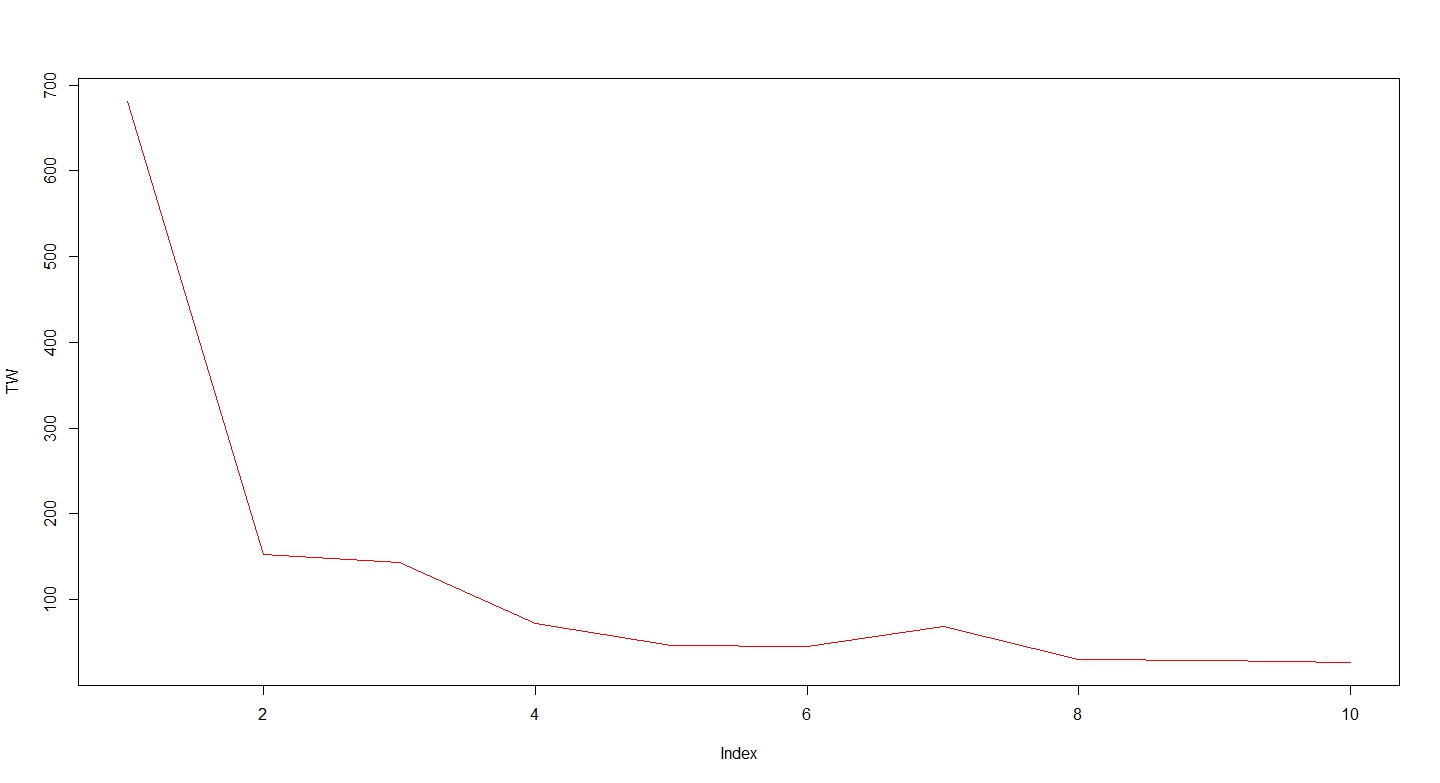
\includegraphics[width=1.1\linewidth]{./Scree}

\end{figure}

\end{document}